\section{Introduction}\label{ch:introduction}

\lettrine[nindent=0em,lines=3]{T} his report details a project done in Wireless Sensor Networks (WSN) with a mini-project called "To hop or not to hop". The project follows the original idea of determining when to relay packets in a wireless network, but with a little twist to it - instead of placing the receiving node in a fixed position, we place it on an athlete running a marathon on a oval-formed running track in order to measure his heart rate every minute. This information is going to be transfered to a sink (base station) over a wireless connection with an added two relay stations in between that help ensure sufficient network coverage of the track. To design the track for our purpose, we will employ knowledge of fading, radio wave propagation and received input power (dbM) in a wireless node.

\noindent We will seek to create an effective protocol that can determine when to communicate directly with the node carried on the athlete/runner and when it is best to use one of the relays. This protocol will take signal strength into consideration. For inter-node connectivity, we will design and implement the data-link layer stop-and-wait ARQ method on all nodes.\footnote{\cite{Ieee}}

\noindent With reference to the mini-project presentation, we use telosb nodes all running TinyOS with a packet size of 128 bytes. The RF transceiver is a single-chip 2.4 GHz IEEE 802.15.4 compliant CC2420 with a data rate of 250 kbps.

\noindent Section \ref{ch:theory} details the theory behind the implementation in section \ref{ch:implementation}. Set in a real-life scenario, we performed a test of the WSN with results in section \ref{ch:results}. The conclusion of our project is in section \ref{ch:conclusion}.

\begin{figure}[h]
	\centering
	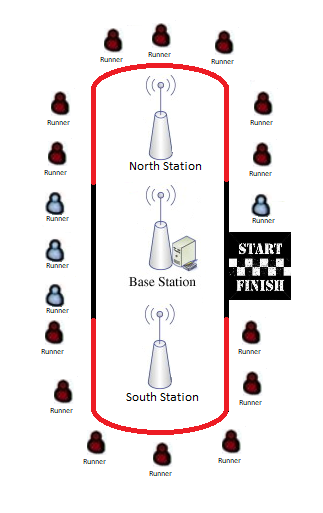
\includegraphics[width=1\linewidth]{introduction/scenario/fig/scenarioIntroduction.png}
	\caption{A base station requests heart rate information from a marathon runner racing around a track. In the red northern territory, the runner is out of range, so the base station transmits requests to the north station which relays the message and likewise with the south station.}
	\label{fig:scenarioIntroduction}
\end{figure}